%------------------------------------------------- 
\subsection{Discovery Strategy}
\label{subsec:fit_bh}

Model-independent fits for the discovery region are performed using \textsc{pyBumpHunter} \cite{bumphunt}.
The strategy consists of comparing the data in a given \mt~spectrum to a background estimation derived by performing the polynomial fit.
This allows the background estimation method for the Discovery strategy to remain the same as for the SVJ Fit strategy, but introduces a bump hunt for model independent signal interpretation. 

The polynomial fit is done to an \mt~distribution with 180 bins (25 GeV wide), which is half the width of the bins used in the SVJ Fit strategy (50 GeV wide). %90 bins, as with the PFN 
The narrower bins allow for rebinning based on the \textit{signal mass resolution} of the SVJ signals.
The binning strategy is outlined in Appendix~\ref{app:binning}.

Figure~\ref{fig:bkgfit_data_crvr_antelope} shows the fit and residuals of the polynomial with the narrower binning in the CR and the Discovery VR data.
Table~\ref{fig:postfit_param_antelope} shows the post-fit values of the fit parameters and their uncertainties for the CR and VR. 
These results indicate good ability of the 5-parameter polynomial to model the ANTELOPE selected data.

\begin{figure}[!htbp]
\centering
   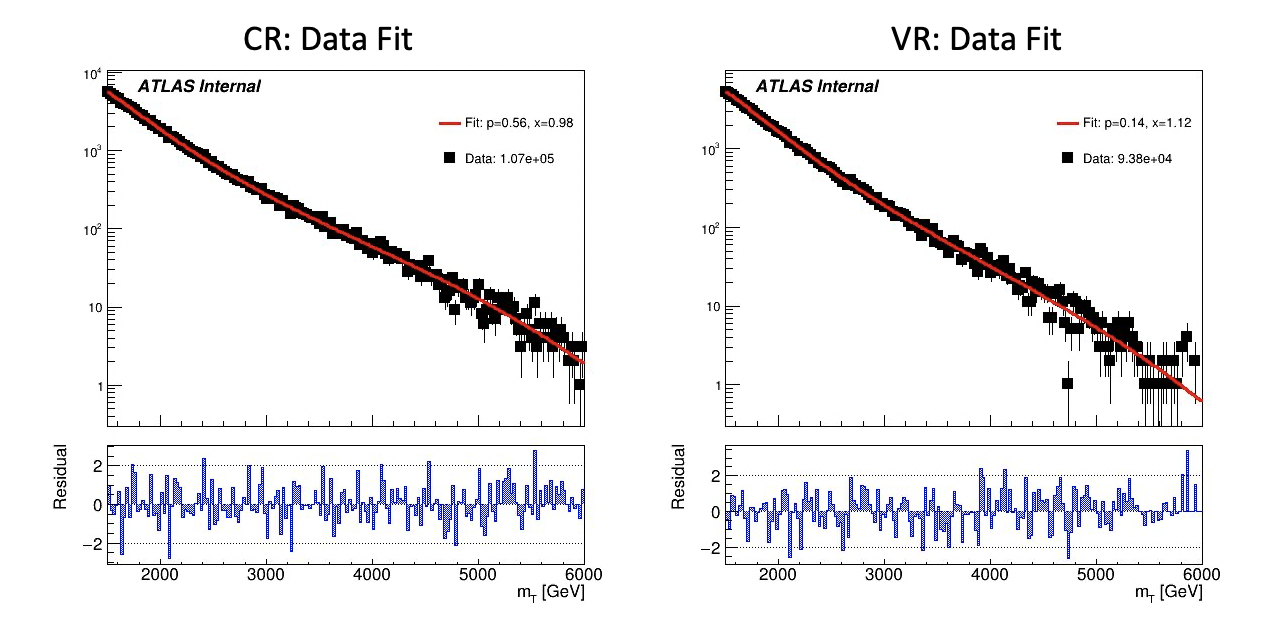
\includegraphics[width=0.95\textwidth]{figures/stats/bkgfit_data_crvr_antelope}
    \caption{Post-fit function and residuals for the ANTELOPE CR and VR.
    \label{fig:bkgfit_data_crvr_antelope}}
\end{figure}

\begin{table}[!htbp]
\centering
   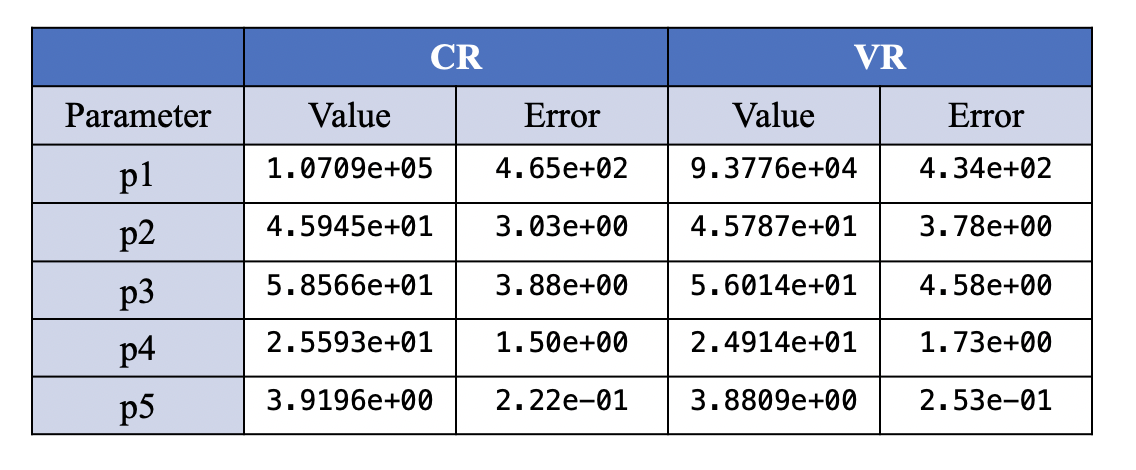
\includegraphics[width=0.65\textwidth]{figures/stats/postfit_param_antelope}
    \caption{Post-fit parameters for the ANTELOPE CR and VR.
    \label{fig:postfit_param_antelope}}
\end{table}

The studies previously shown in Section~\ref{subsec:fit_bkgonly} validate the robustness of the background polynomial fit. 
The narrower bins are the only difference for polynomial fitting between the SVJ Fit and Discovery Fit strategies, and they are not observed to reduce the quality or consistency of the fit. 

%----------------------------------------------------------------------------------------
\subsubsection{BumpHunter Fits}
\label{subsec:bhfits}

The signal mass resolution binning strategy described in Appendix~\ref{app:binning} creates a monotonically increasing set of bins. 
While the SVJ signals help inform the binning, the binning is still broadly applicable to a variety of potential signal models.
The mass resolution of any resonant signal generally widens as the mass of the mediator particle increases.
A similar strategy and binning was used in the generic heavy resonance search presented in Ref.~\cite{yxh}.
The resulting set of 15 bins to be used in the BumpHunter (BH) fits varies in width from 100 GeV at the \mt~core to 925 GeV in the \mt~tail. 

Figure~\ref{fig:antelope_bh_crvr} shows the result of running BumpHunter over the rebinned CR and VR \mt~spectra.
The background estimation is given by the polynomial fit function. 
The BH $p$-values (>0.05) indicate agreement with the background estimation.
The BH $p$-value for the VR is somewhat low at 0.07, but within the realm of statistical fluctuations, and is thus not a cause for concern.
The $p$-value of the polynomial fit which gives the background estimation is also reported.
The location of the largest bump identified by BH is indicated on the plot. 
\begin{figure}[!htbp]
\centering
   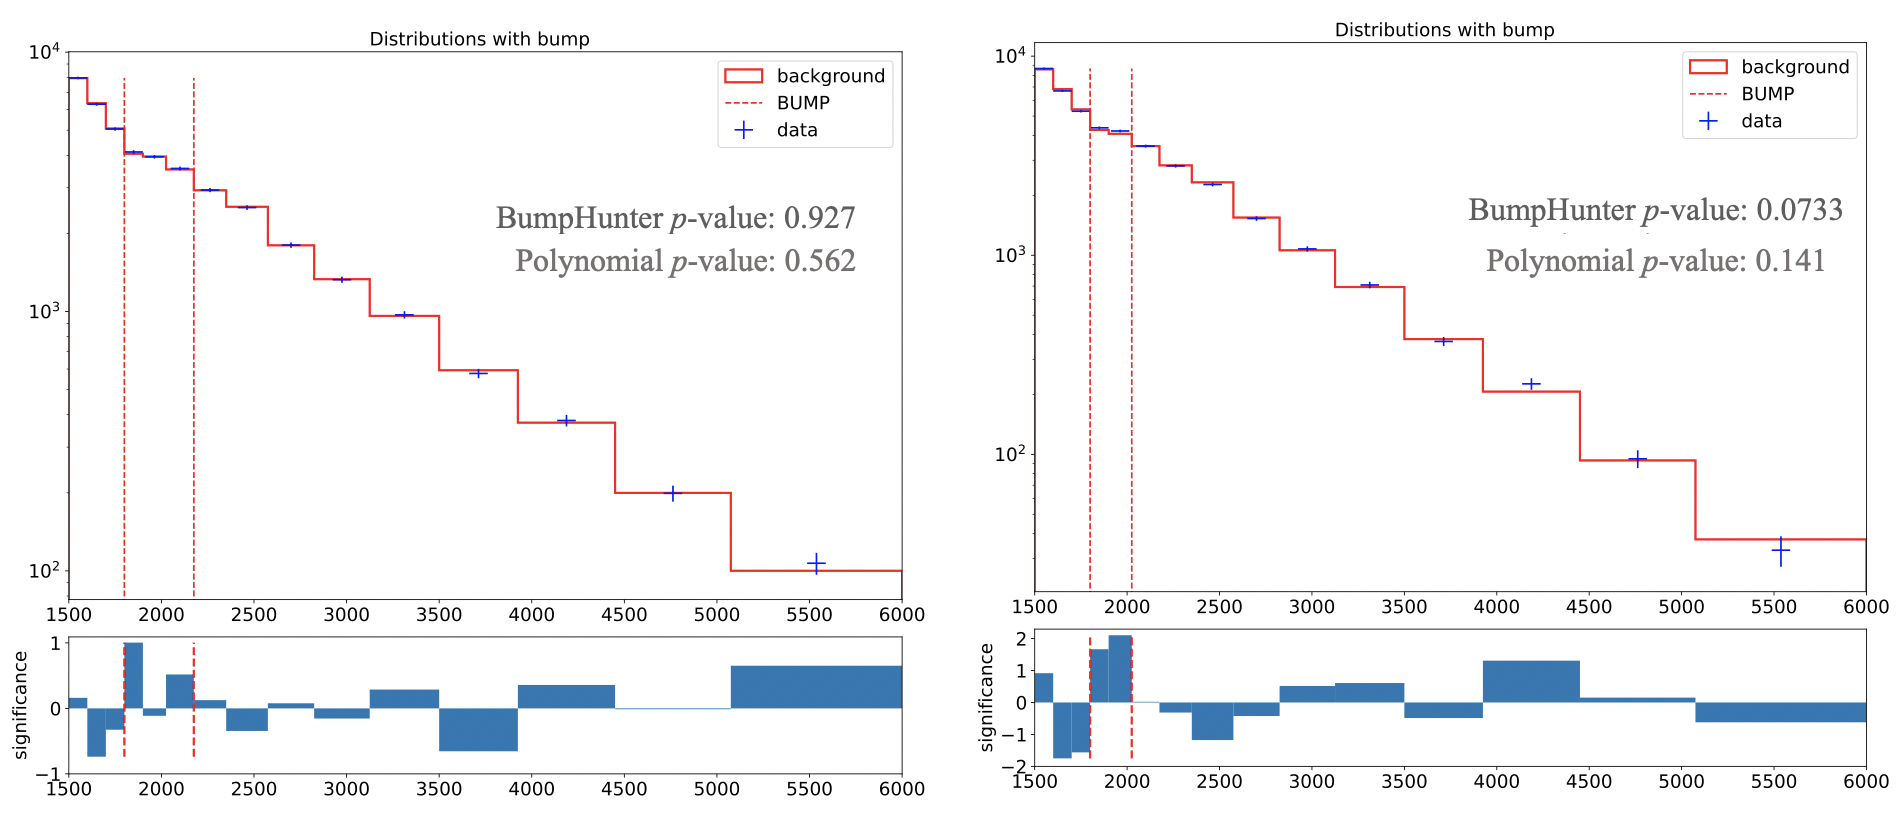
\includegraphics[width=0.95\textwidth]{figures/stats/antelope_bh_crvr}
    \caption{BumpHunter fits on the ANTELOPE \mt~spectra for both the CR (left) and VR (right). In a signal-depleted region, good agreement with the background estimation is observed.
    \label{fig:antelope_bh_crvr}}
\end{figure}

Figure~\ref{fig:bh_asimov_pvals} shows BumpHunter $p$-values over 100 Asimov trials, where each toy is scaled to the statistics of the SR.
The agreement is generally very good, as the $p$-values trend towards higher values.
Since there is an upward trend in the $p$-values rather than a flat distribution as seen for the polynomial fit, we can conclude that the background estimation captures the data slightly ``too well'', reducing the frequency of low $p$-value BH fits.
This indicates that some signal sensitivity (or ability to detect distributions with poor data/background agreement) is lost to the over-performant background estimation.
This is accounted for in the signal injection studies presented in the next section, and ultimately was determined to not pose a significant issue for the analysis strategy.
While the $p$-value distribution is not flat, we do see some fits with $p$-value < 0.10, indicating that low $p$-values are still possible from a background only distribution.
No fits with a \textit{spurious signal} are found.
A spurious signal would be indicated by a fit with a BH p-value $<$ 0.01 or a maximum local significance of > 2$\sigma$.
\begin{figure}[!htbp]
\centering
   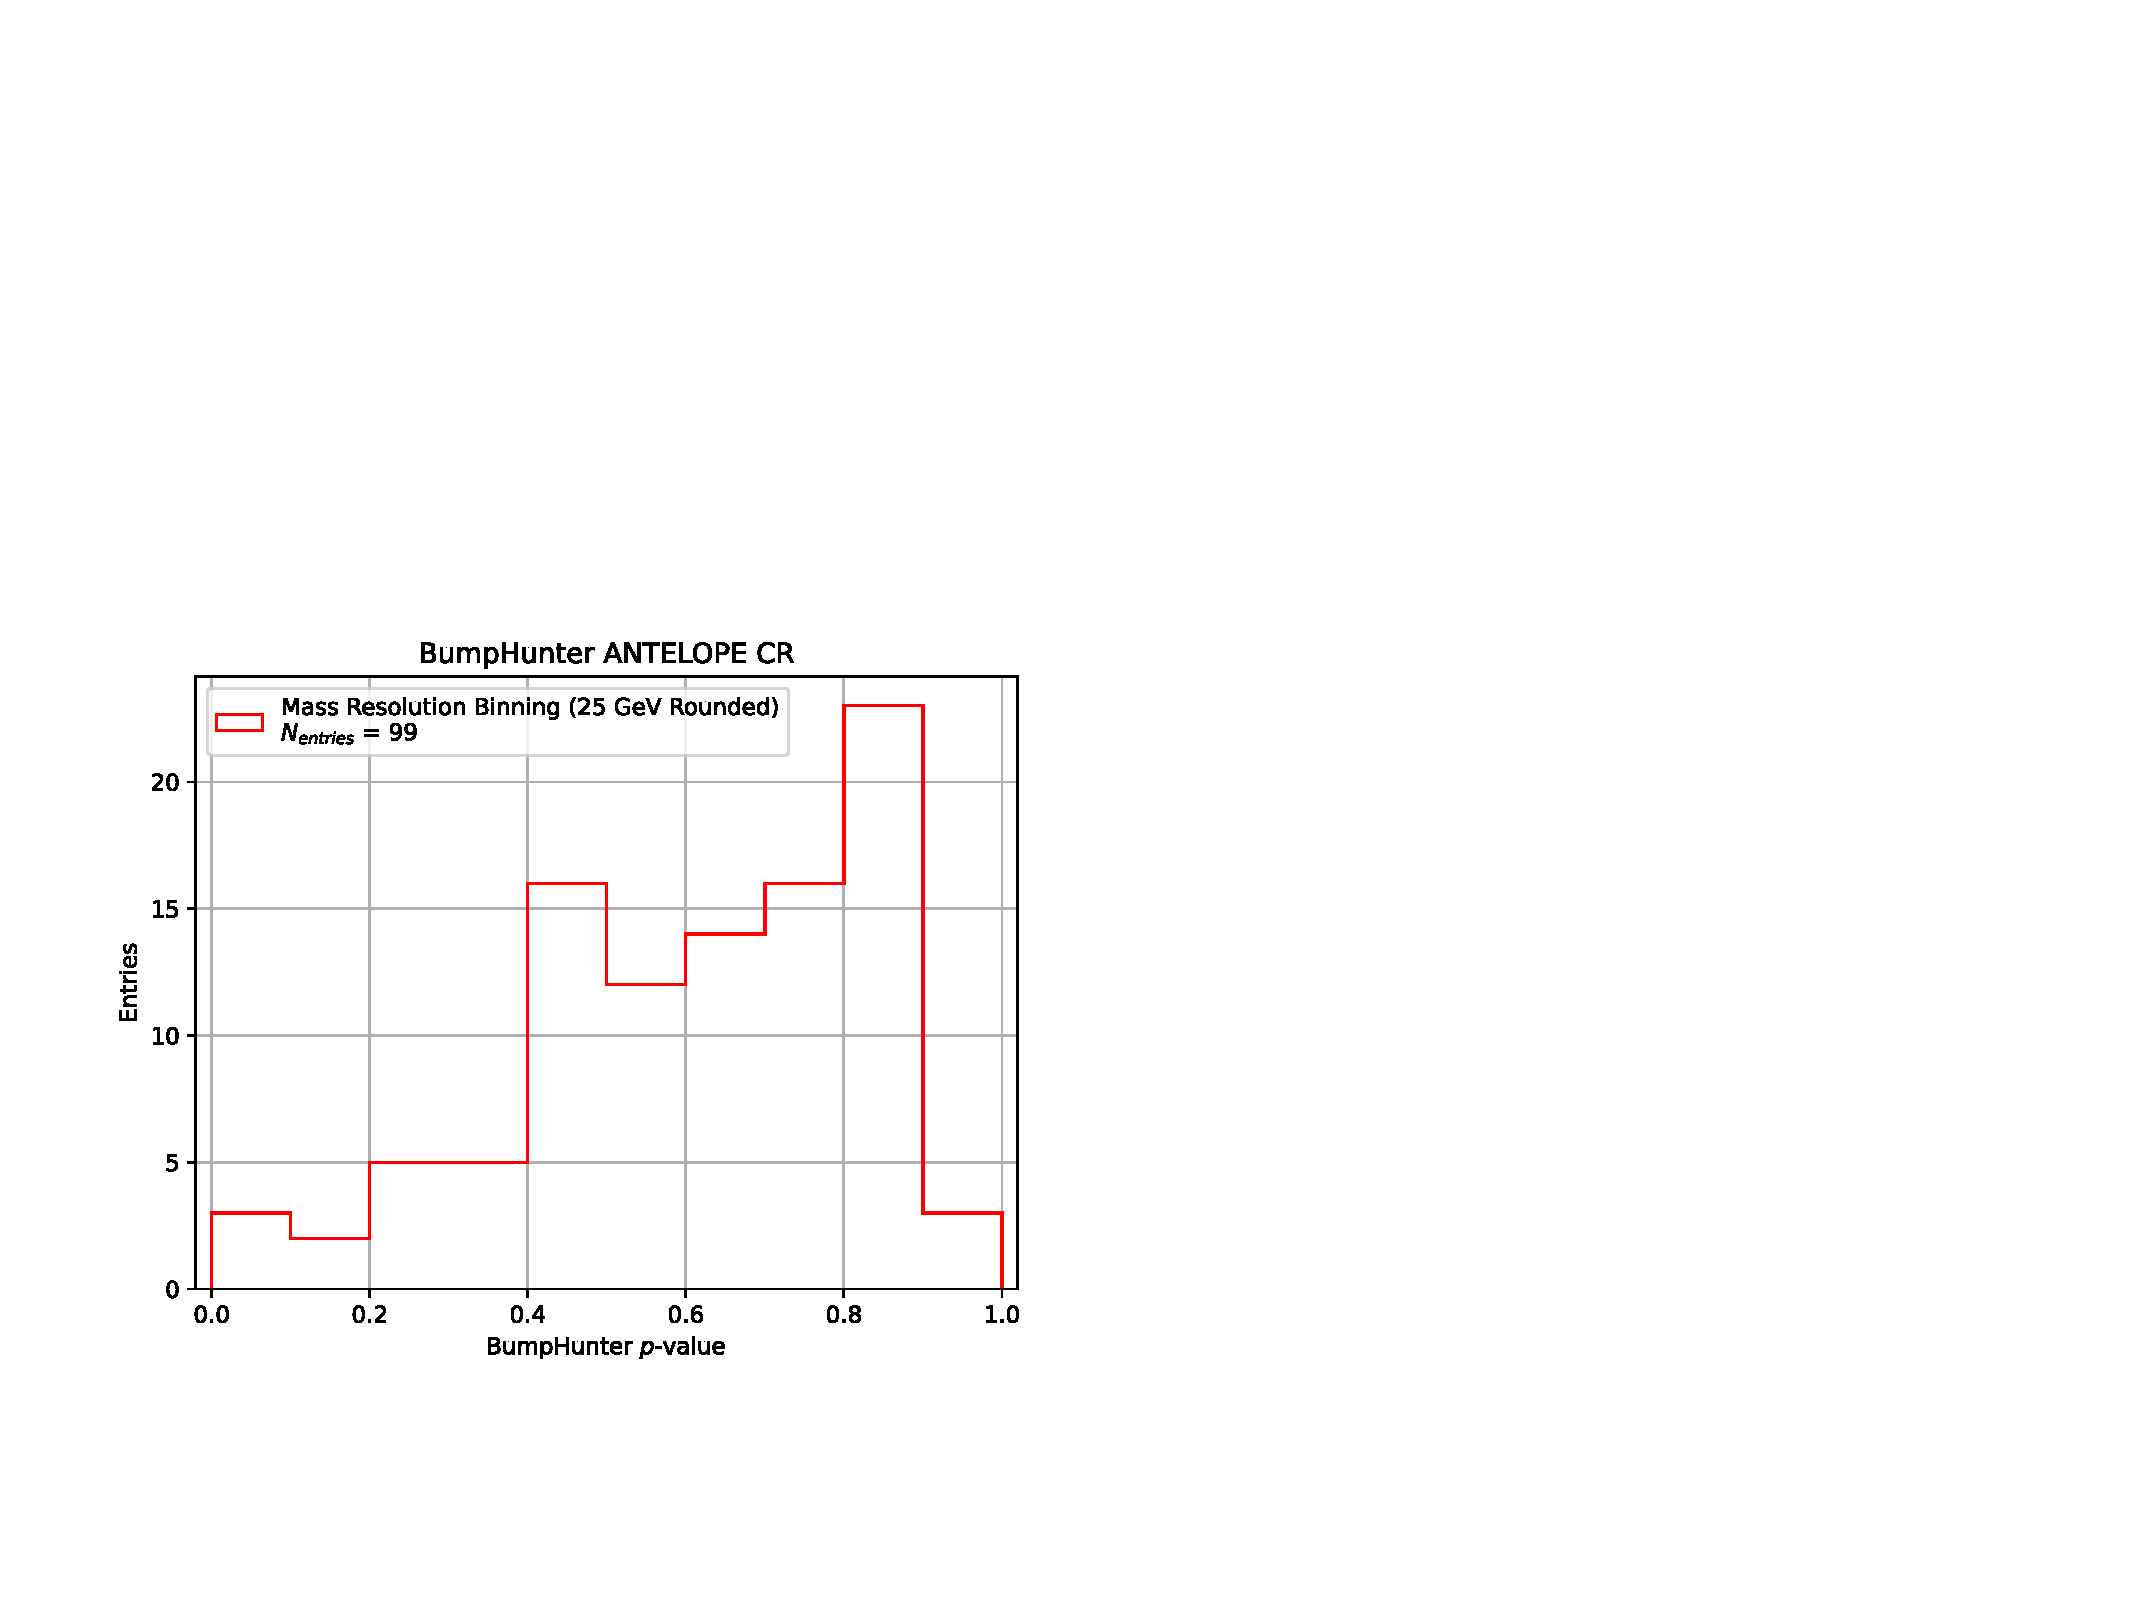
\includegraphics[width=0.45\textwidth]{figures/stats/bh_asimov_pvals_cr}
   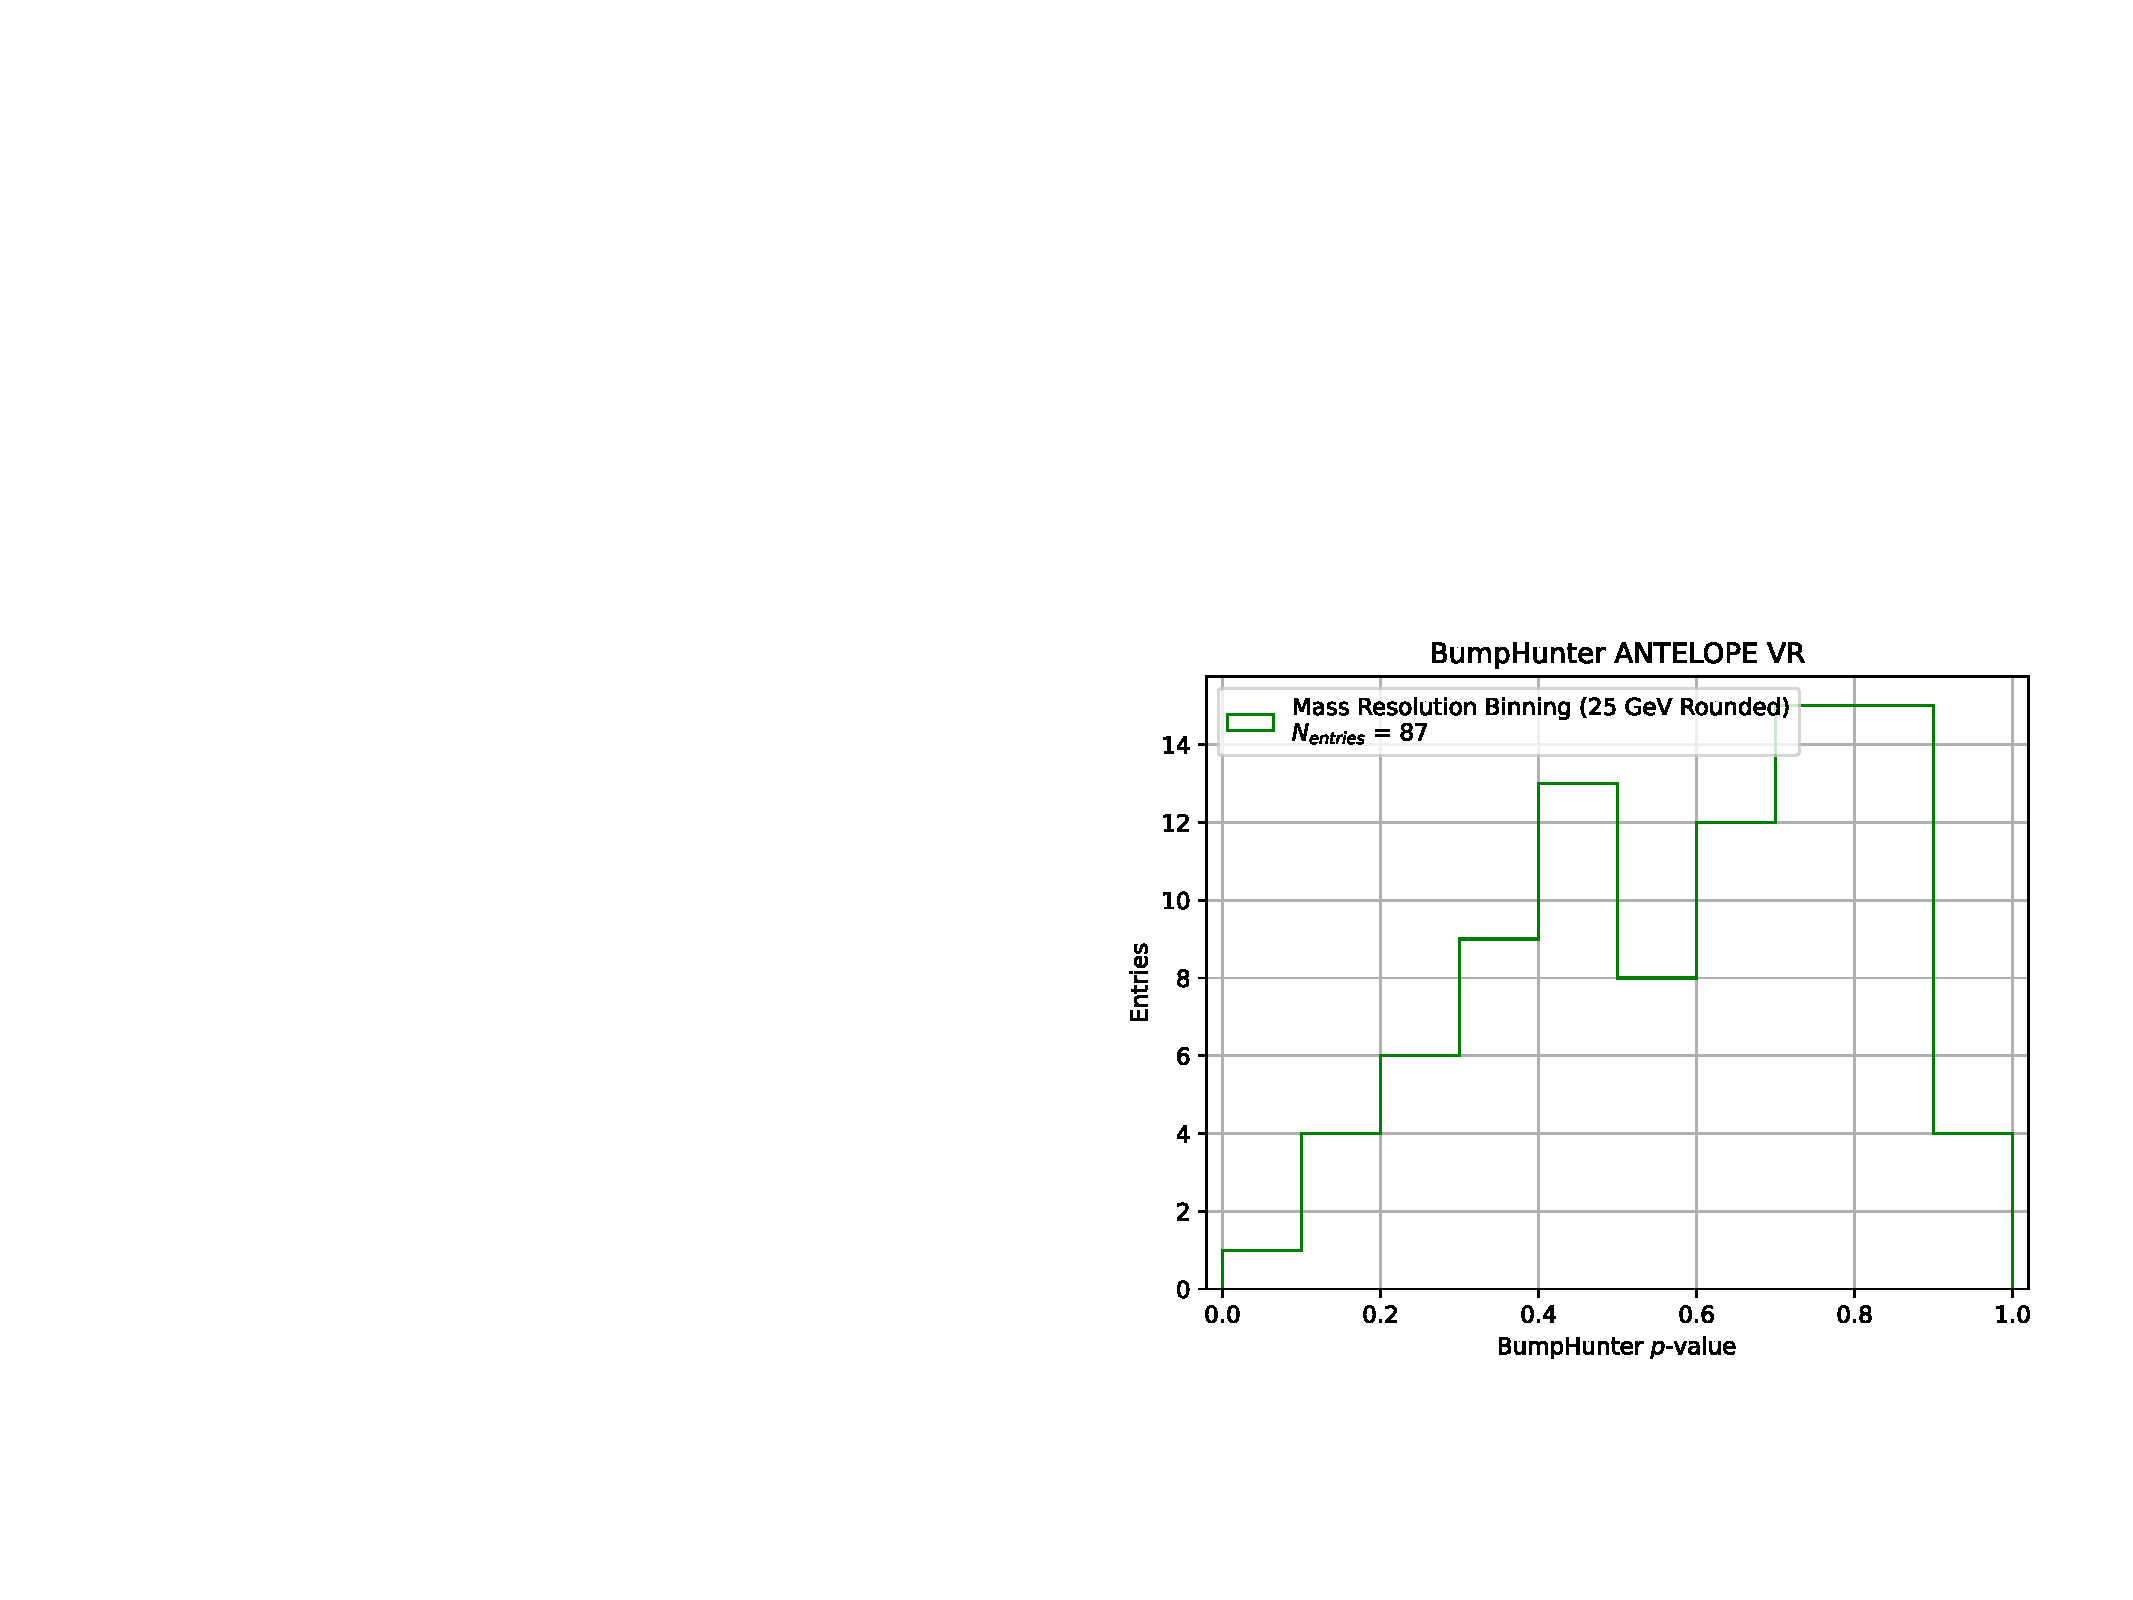
\includegraphics[width=0.45\textwidth]{figures/stats/bh_asimov_pvals_vr}
    \caption{BumpHunter p-values extracted for 100 Asimov toys for both the ANTELOPE CR (left) and VR (right). Fits where the polynomial fit initially failed to converge are excluded from the plot. These fits were later recovered through modification of the initial parameters.
    \label{fig:bh_asimov_pvals}}
\end{figure}

%----------------------------------------------------------------------------------------
\subsubsection{BumpHunter Signal Injection}
\label{subsec:bhsiginj}

To explore a model independent signal hypothesis, signal injection tests in the ANTELOPE region are done with generic Gaussian shapes.
Two Gaussian models are built with a mean ranging from 2000 GeV to 5000 GeV and a standard deviation (or \textit{width}) equal to 10 or 20\% of the mean value.
Figure~\ref{fig:gauss_inj} illustrates an injected Gaussian and its effect on the \mt~distribution.
The 20\% gaussian represents the widest possible signals we might be sensitive to with a BH strategy, while the 10\% injection represents a narrower signal peak. 
As the SVJ model and other dark QCD models generally predict wide signal shapes due to the presence of \met~in the final state, narrower Gaussians were not explored.

\begin{figure}[!htbp]
\centering
   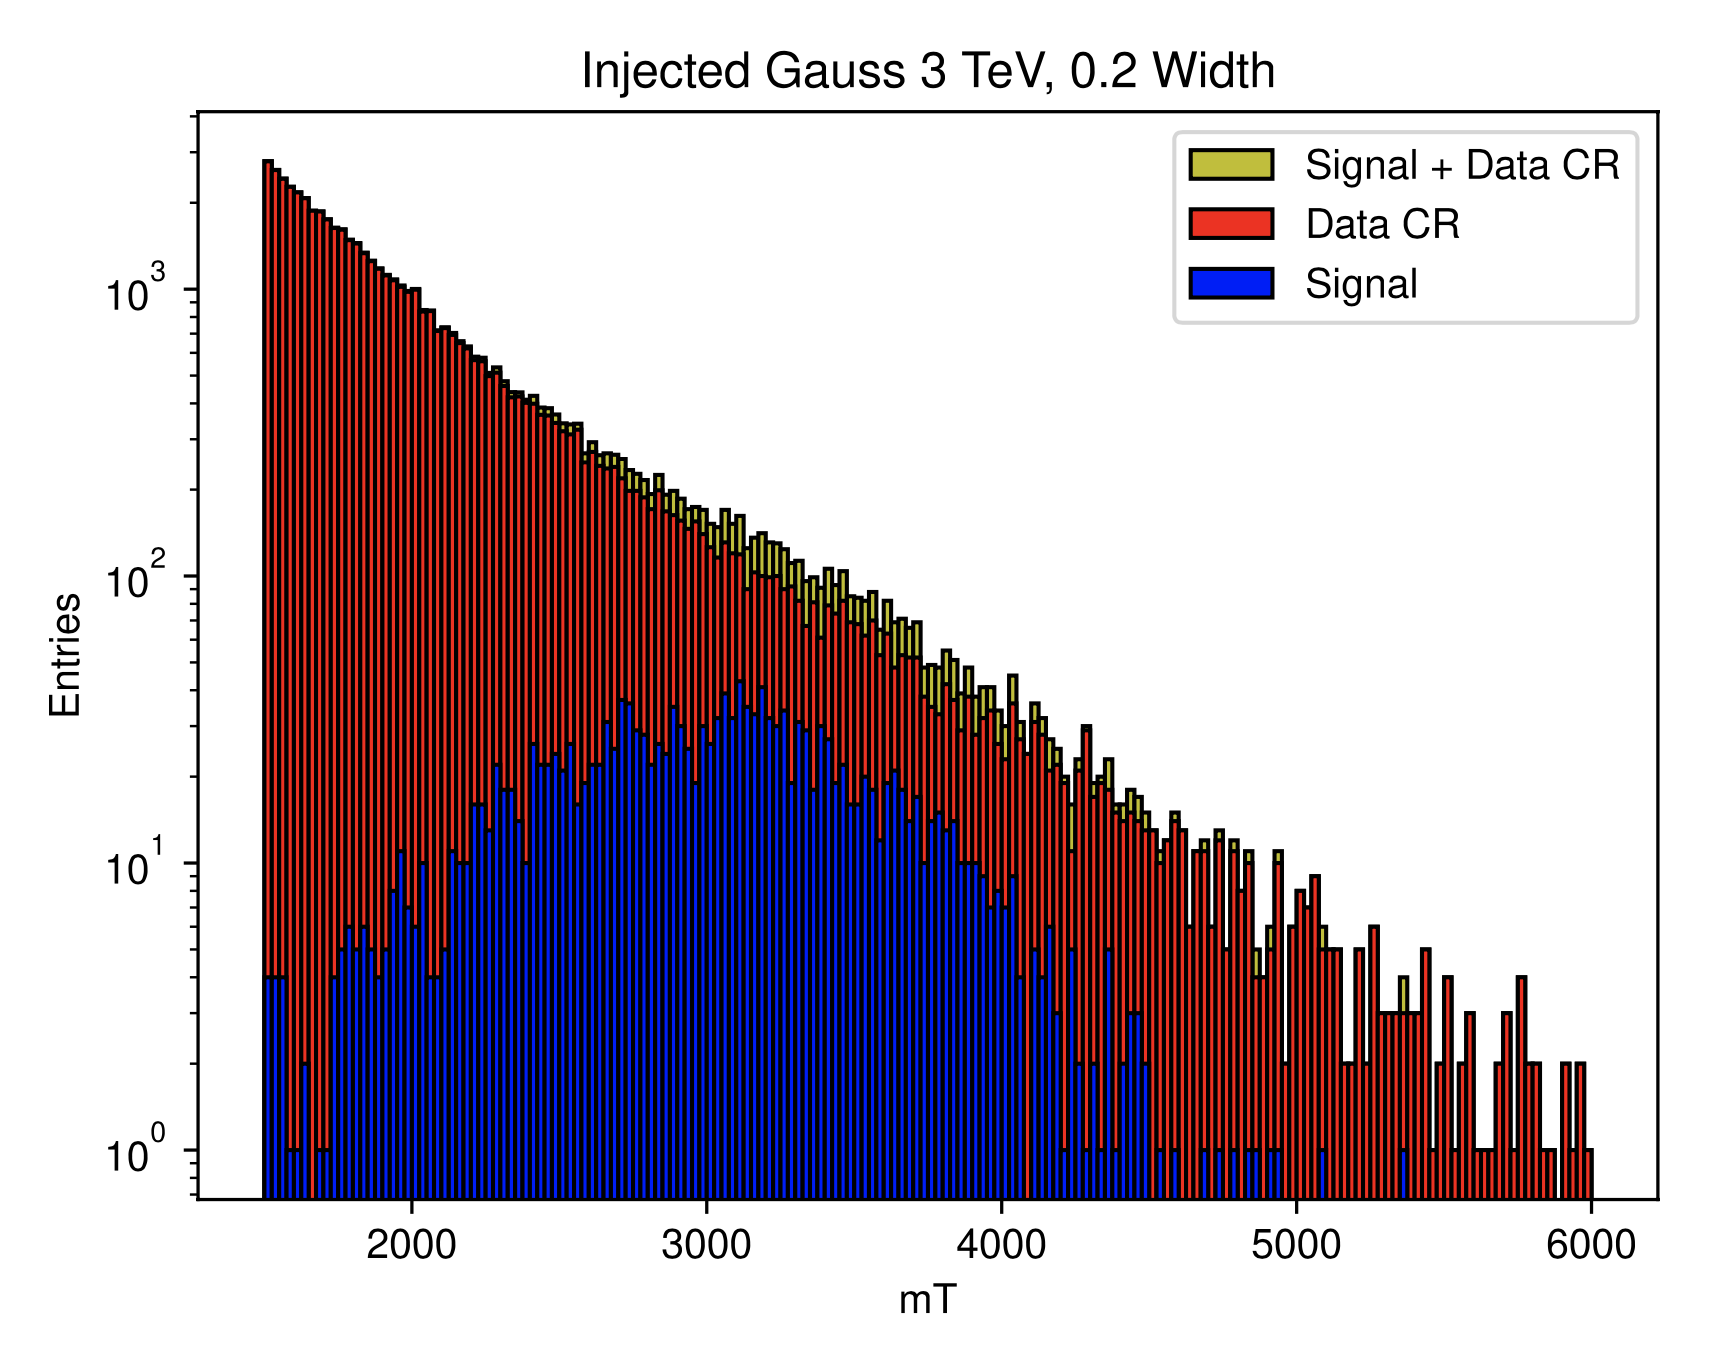
\includegraphics[width=0.5\textwidth]{figures/stats/gauss_inj}
    \caption{Example injected gaussian signal, with mean = 3000 GeV and width of 20\%.
    \label{fig:gauss_inj}}
\end{figure}

%The polynomial fit framework is run over background-only Asimov data to determine the injection level, as discussed in Section~\ref{subsec:fit_expsens}. 
%It should be noted that the $5\sigma$ injection level as determined by the polynomial fit is an underestimate, as the flexibility of the fit absorbs some of the signal.

An estimated $5\sigma$ of signal is injected for these tests.
The estimate is derived from the amount of signal necessary to produce a 5$\sigma$ excess in the polynomial fit.
It is an underestimate of the expected significance to the BumpHunter, as the flexibility of the background-only polynomial fit absorbs some of the signal.
Therefore we do not expect to measure $5\sigma$ significance with the BH approach, but rather hope to see that some level of signal (at least $\geq2\sigma$ local significance) is observed by the BumpHunter method.

Results are obtained by averaging over 100 toys for each injection.
Figure~\ref{fig:siginj_bh} shows the resulting maximum local significance and the location of the determined bump, indicating a good response of the BumpHunter framework for detecting generic \mt~resonances at the right location.
Only the 5000 GeV 20\% width point is not properly identified by the framework. 
While some sensitivity is lost due to the flexible nature of the fitting framework, the ability to identify a bump with substantial local significance in the correct location is observed.
Figure~\ref{fig:bh_bump_example} shows an example of the identified bump.

\begin{figure}[!htbp]
\centering
   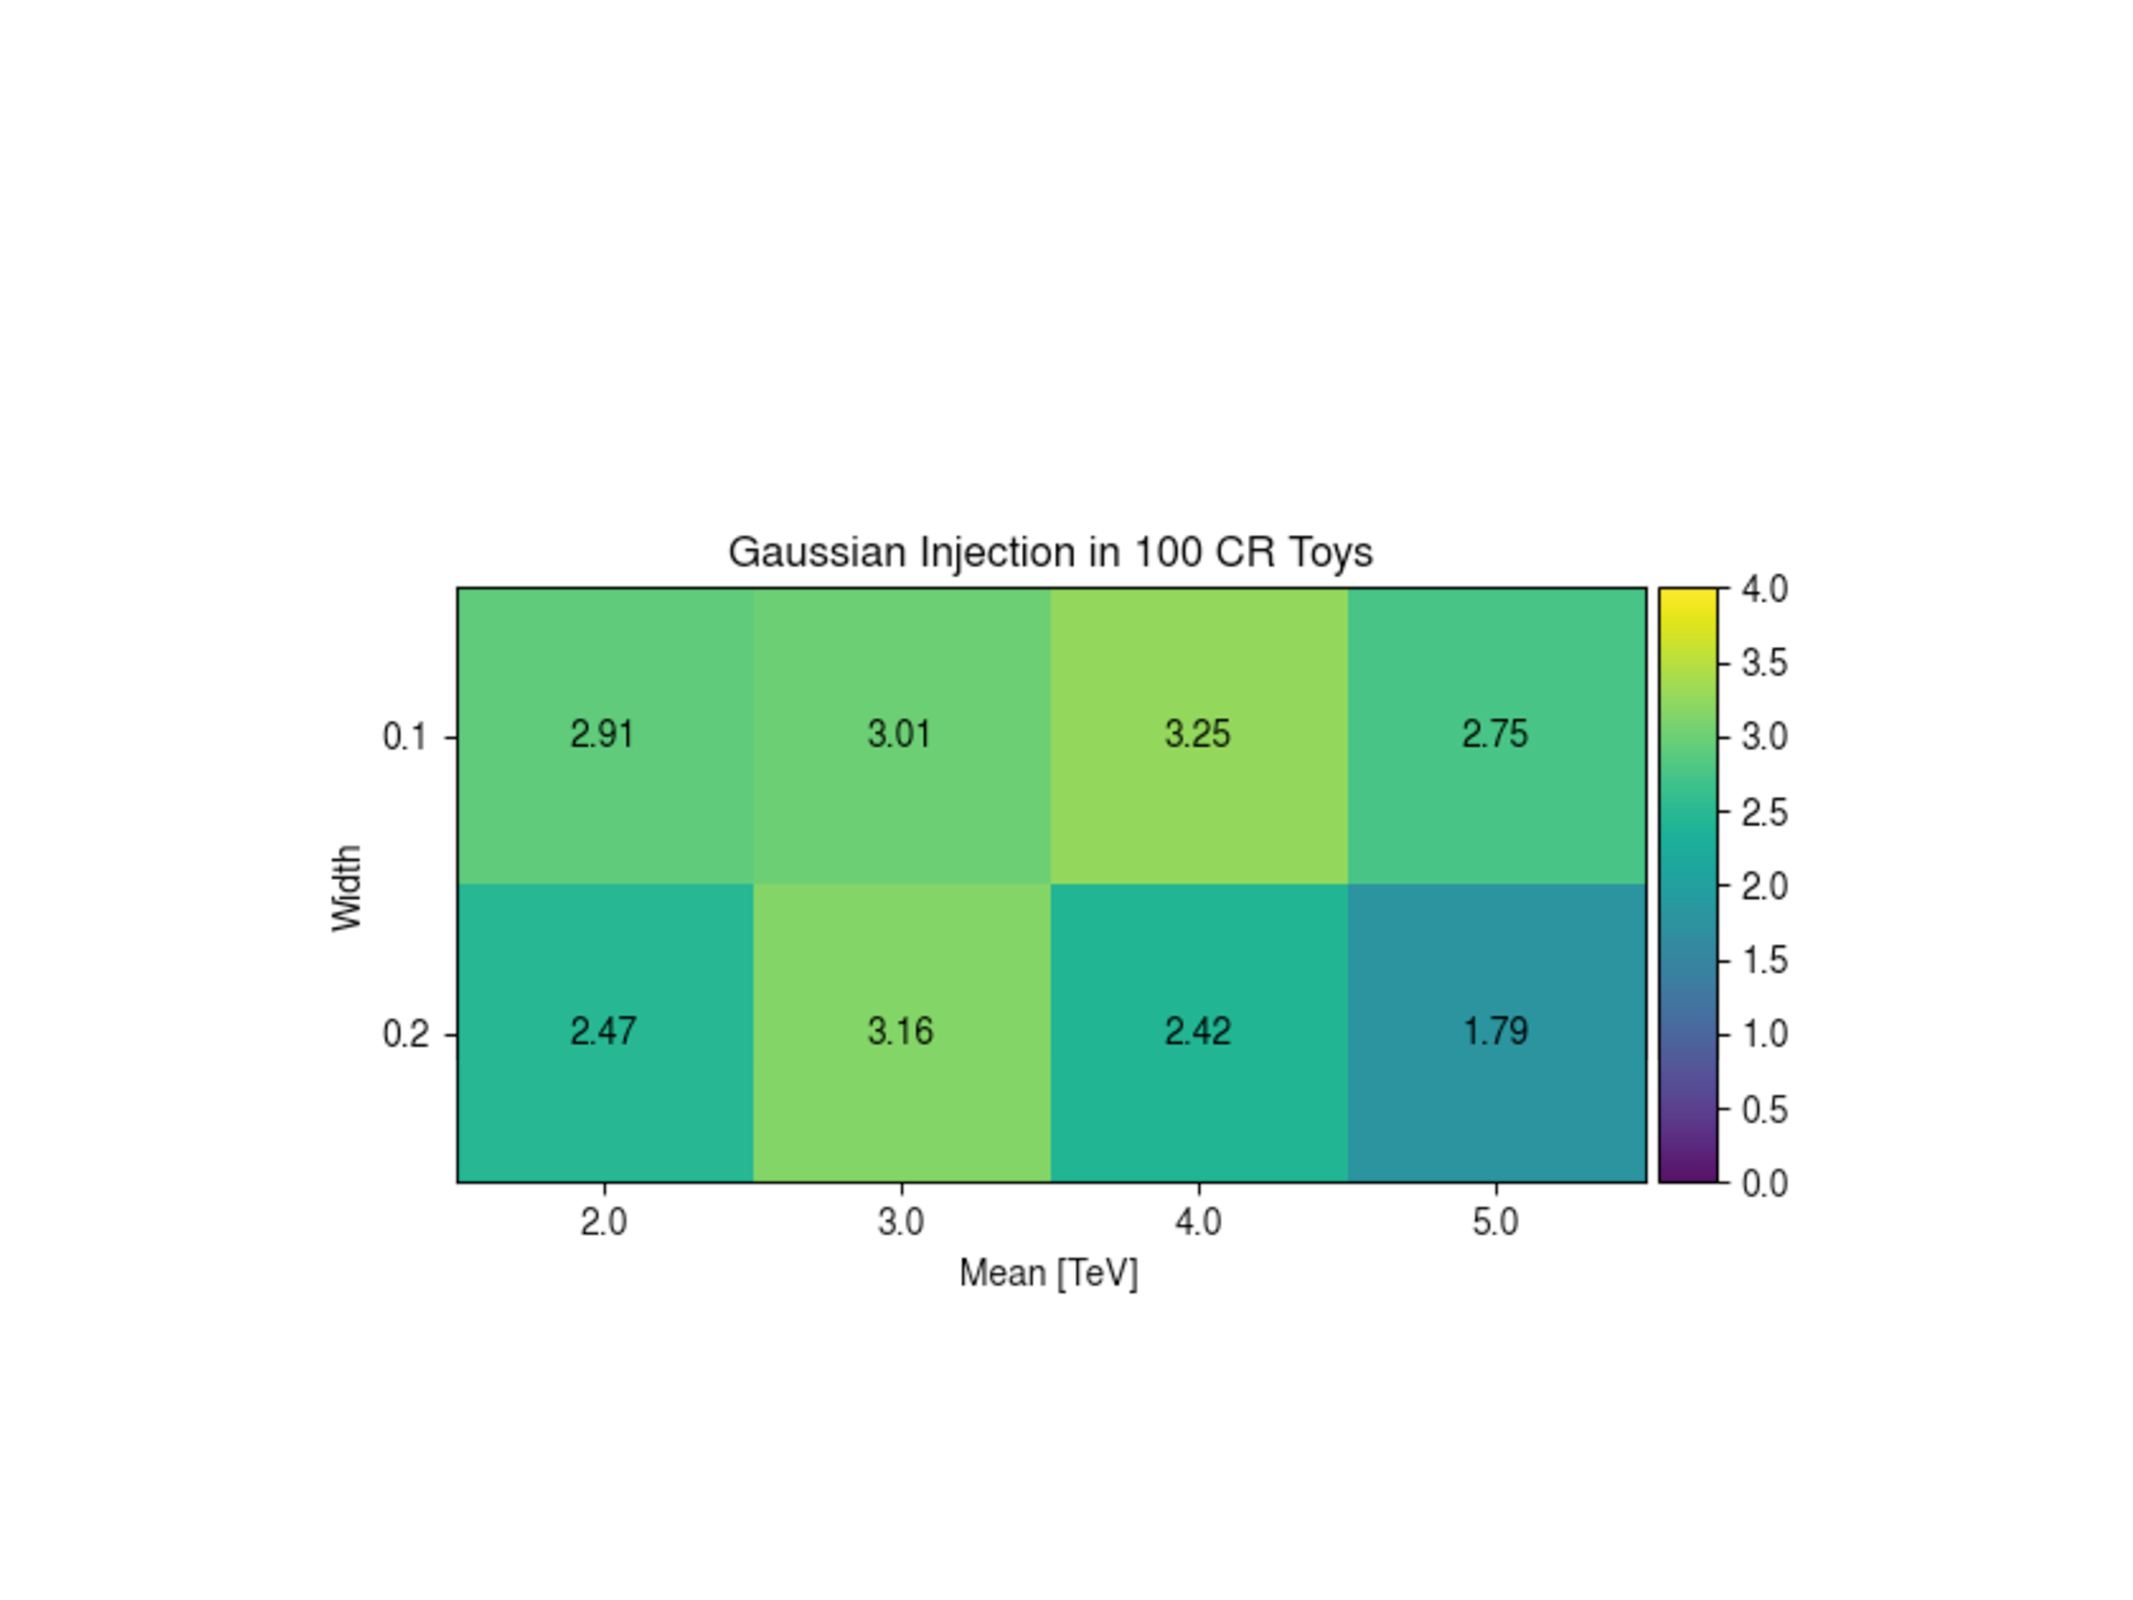
\includegraphics[width=0.65\textwidth]{figures/stats/siginj_bh_localsig.pdf}
   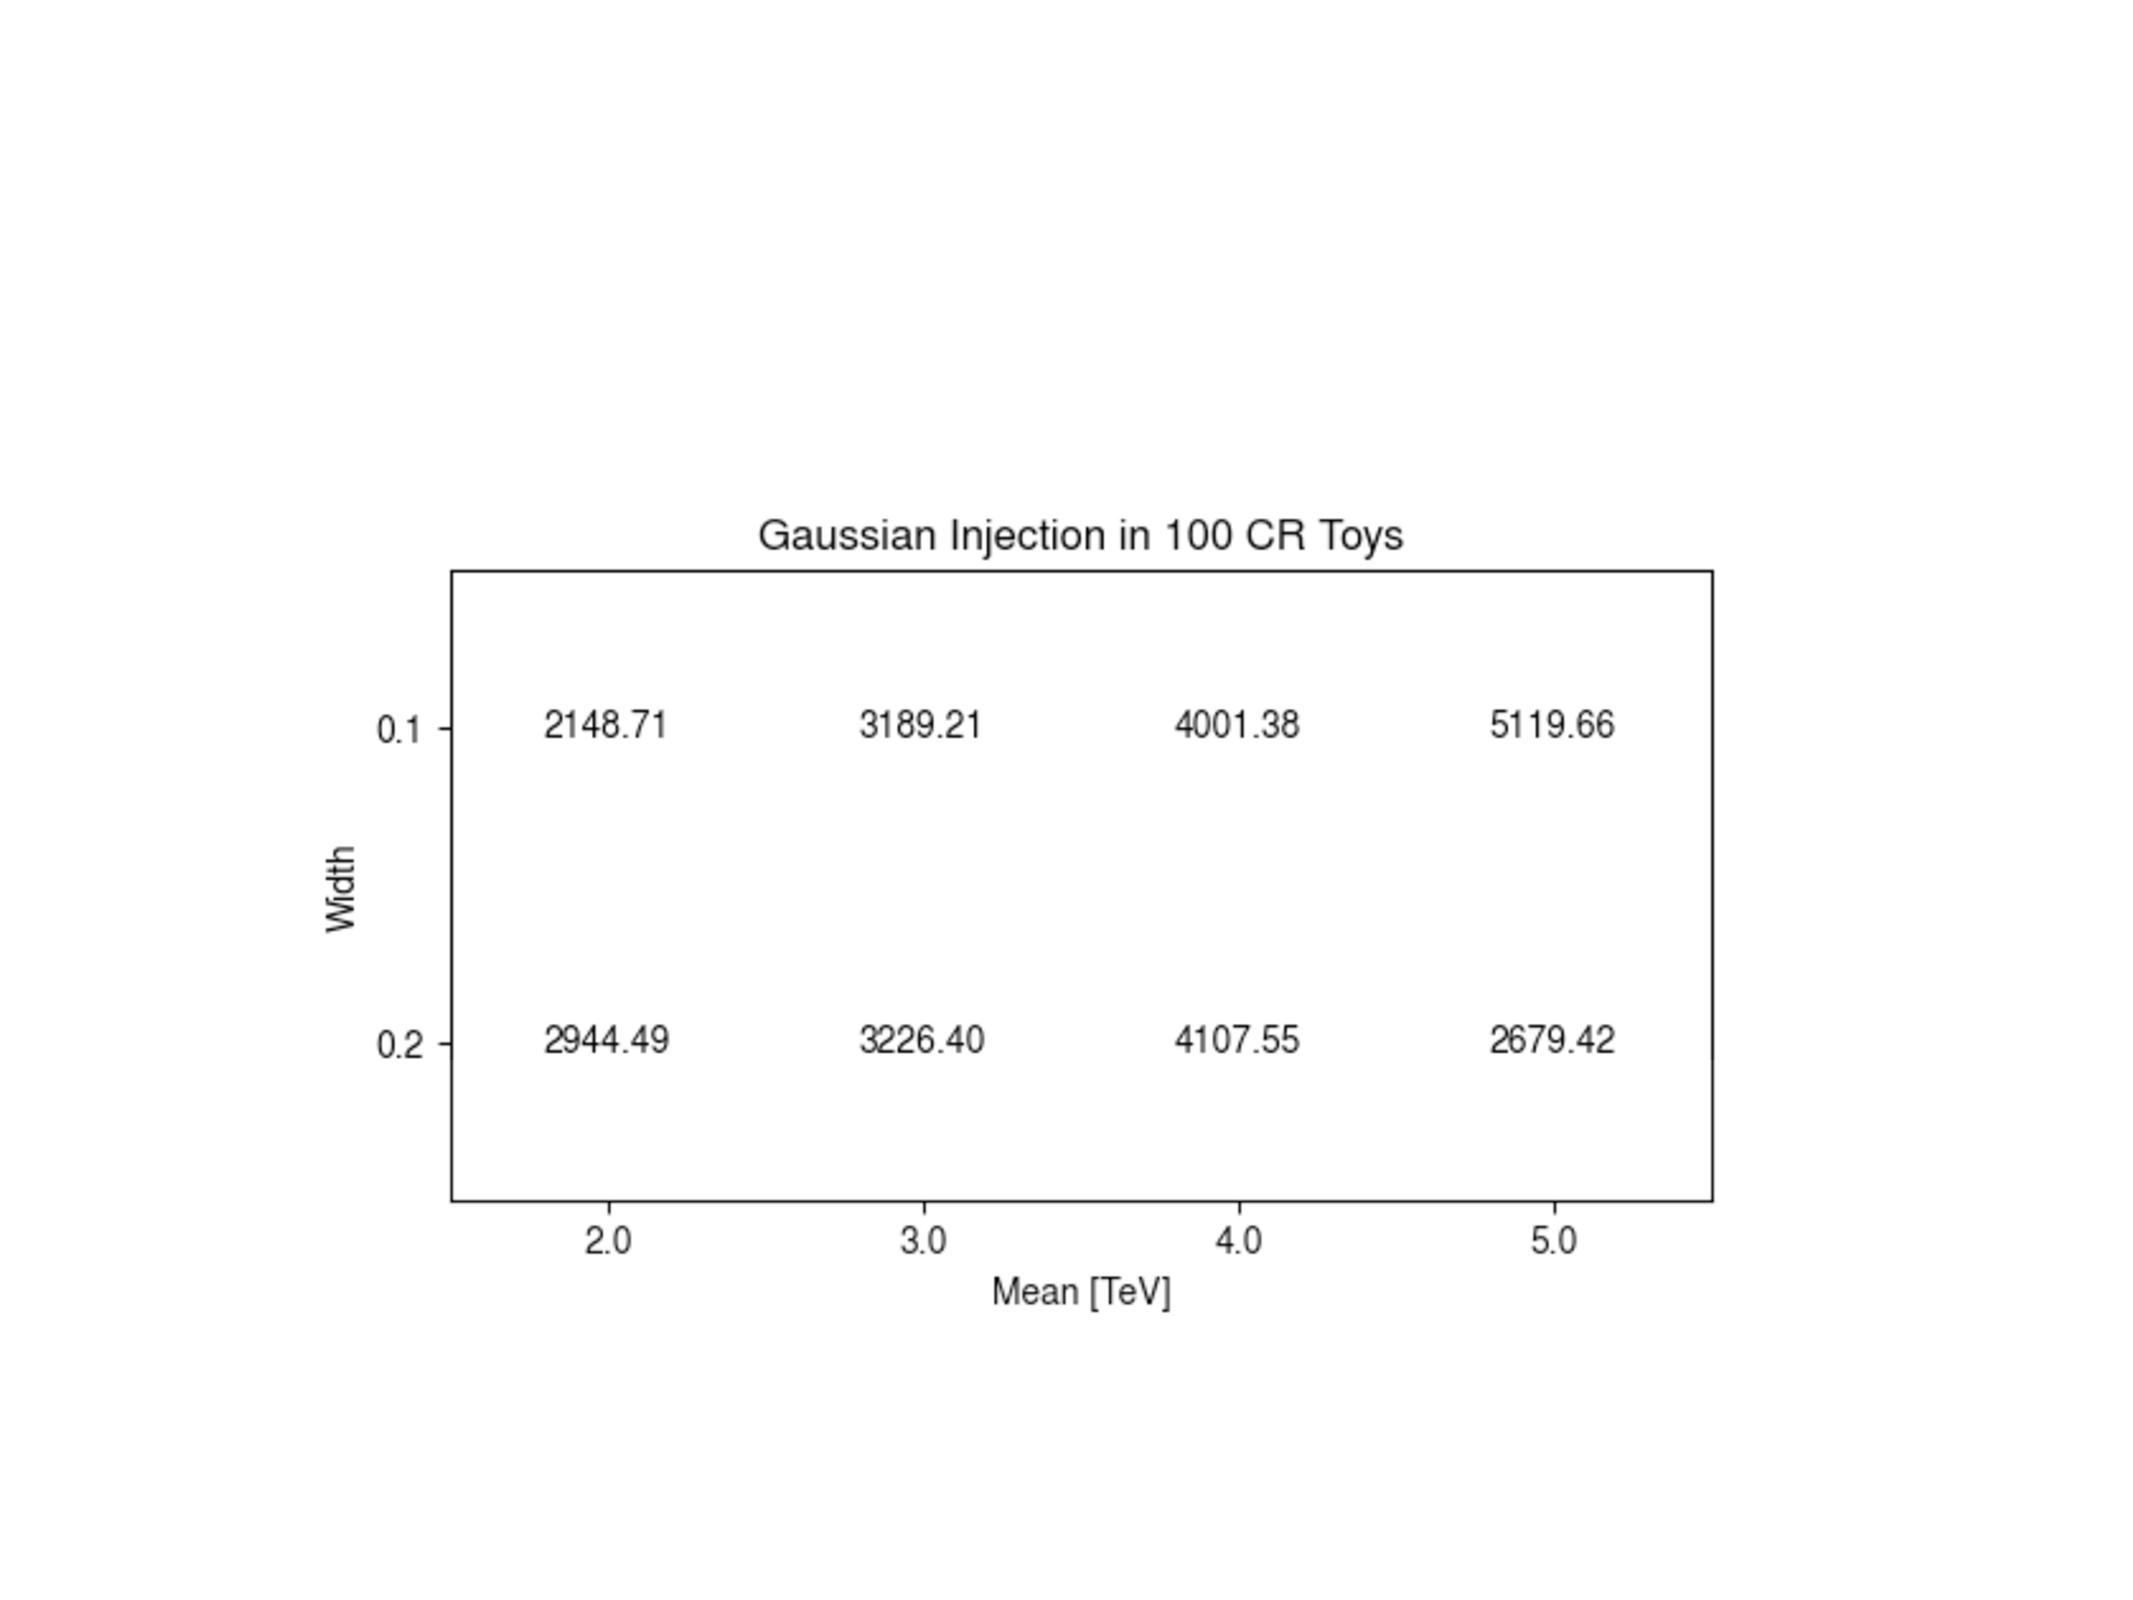
\includegraphics[width=0.65\textwidth]{figures/stats/siginj_bh_bumploc.pdf}
    \caption{Response of the BumpHunter framework to gaussian signal injection is shown. The local significance (top plot) and bump location in GeV (bottom plot) are shown. With the exception of the 5.0 TeV 20\% width signal (expressed as 0.2), the BH identifies bumps with a significance > 2.0$\sigma$ in approximately the correct location.
    \label{fig:siginj_bh}}
\end{figure}

\begin{figure}[!htbp]
\centering
   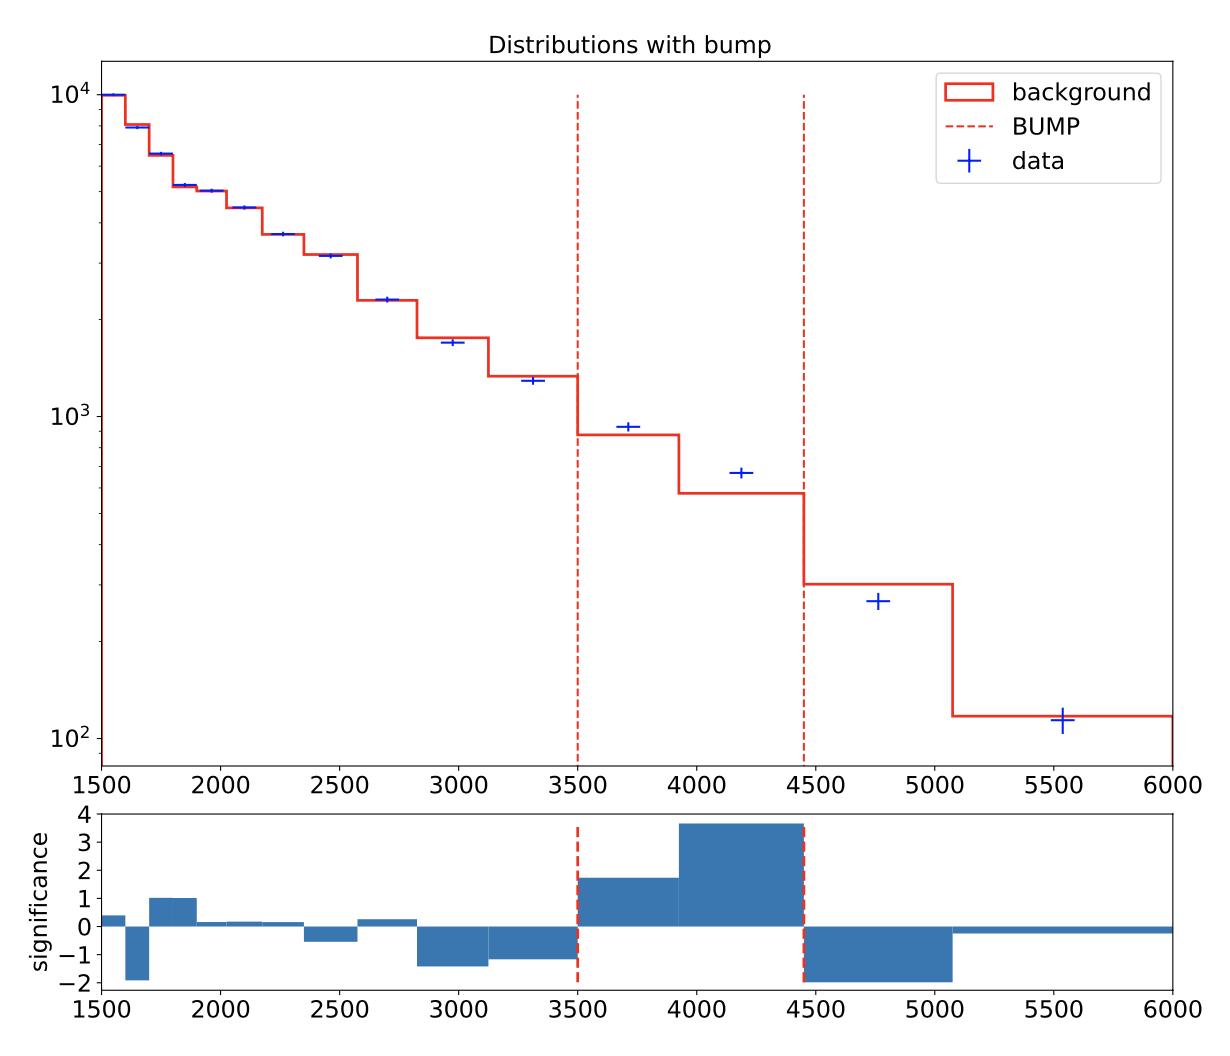
\includegraphics[width=0.5\textwidth]{figures/stats/bh_bump_example}
    \caption{Example BH response to gaussian signal injection at 4000 GeV with width of 10\%. 
    \label{fig:bh_bump_example}}
\end{figure}

%The BH significance can be slightly enhanced by repeating the polynomial fit after blinding the the most significant bump.
%This serves to ``flatten" the fit, allowing the bump to be more significant compared to the the background distribution. 
%This process is illustrated in Figure~\ref{fig:bh_masked}. 
%This strategy has the potential impact of enhancing non-signal deviations in the fit as well.
%Therefore, both BH results are considered together.

%\begin{figure}[!htbp]
%\centering
%   \includegraphics[width=0.95\textwidth]{figures/stats/bh_mask_before.pdf}
%   \includegraphics[width=0.95\textwidth]{figures/stats/bh_mask_after.pdf}
%    \caption{Improvement of the BH response after masking the region []redoing the polynomial background fit
%    \label{fig:siginj_bh}}
%\end{figure}
